\section{Componentes do Beaglebone Black}
\label{ch:bbb_components}

No capítulo \ref{ch:introduction} foi introduzido o Beaglebone Black como um mini computador de arquitetura ARM. Esta seção irá mostrar os componentes da placa e os integrados ao SOC Sitara AM335x. Na figura \ref{figura:bbb_components} tem-se uma foto de frente e verso da placa de circuito impresso do BBB, identificando os componentes, e na tabela \ref{tab:bbb_components} identifica a função de cada componente na placa. Para complementar na figura \ref{figura:bbb_soc} mostra os componentes integrados ao SOC Sitara AM3358A, este último disponível na \emph{rev.3} deste produto.

\begin{table}[h]
	\centering
	\begin{tabular}[c]{ccm{10cm}}
		No.&Componente&Função\\ \hline
		1&Sitara AM335x&SOC do BBB contendo diversos componentes integrados incluindo a CPU, GPU e PRU.\\
		2&HDMI Framer&Converte o controlador de LCD do AM335x.\\
		3&Memória RAM&512MB DDR3.\\
		4&eMMC&4GB de memória de armazenamento interna.\\
		5&TPS65217C&Regulador de potência sofisticado com 4 reguladores de tensão LDO controlado por I2C\\
		6&Ethernet PHY&Conecta o processador ARM a conexão física RJ45 com a velocidade de 100Mbit para enviar e 10Mbit para receber.\\
		7&7x LEDs&\emph{Power} LED (azul), 4 \emph{user} LEDs e 2 LEDs (amarelo = dados enviados/ verde = dados recebidos).\\
		8&\emph{Push Buttons}&Liga/Desliga (\emph{Power}), \emph{Reset Button} e \emph{Boot Switch}. Este último seleciona se o deve ser feito \emph{boot} do eMMC ou do cartão micro SD.\\
		9&Micro HDMI&Para conectar em monitores de até 1280x1024@60Hz ou 1920x1080@24Hz.\\
		10&Ethernet RJ45&Conector RJ45.\\
		11&5V DC& \emph{Jack} de 5mm para usar o BBB sem precisar alimentar com o cabo USB.\\
		12&\emph{Slot} micro SD& \emph{Slot} para cartão micro SD;\\
		13&\emph{Serial Debug}&Conector de 6 pinos para acessar o terminal através da conexão serial (UART0).\\
		14&USB 2.0 \emph{Client}&Conector mini-USB 2.0 utilizado para conectar o BBB ao computador.\\
		15&USB 2.0 \emph{Host}&Conector USB-A 2.0 para conectar os periféricos do BBB, como \emph{webcams}, \emph{mouse}, teclado e outros. Pode-se utilizar um \emph{hub} USB para conectar mais de um periférico.\\
		16\&17&Expansões P8 e P9&Soquete de pinos de extensão P8 e P9. Cada soquete tem 2x23 pinos totalizando 92 pinos no total.\\
		18&JTAG&Espaço para conector JTAG, bastante utilizado em testes de placas de circuito impresso. Porém, necessita de \emph{software} e \emph{hardware} adicional.\\
		19&Conector de bateria&É possível soldar estes 4 pinos para adicionar um conector de bateria a placa.\\
		\hline
	\end{tabular}
	\caption{Relação dos componentes do BBB de acordo com a figura \ref{figura:bbb_components} \cite{derekbbb}.}
	\label{tab:bbb_components}
\end{table}

\begin{figure}
	\centering
	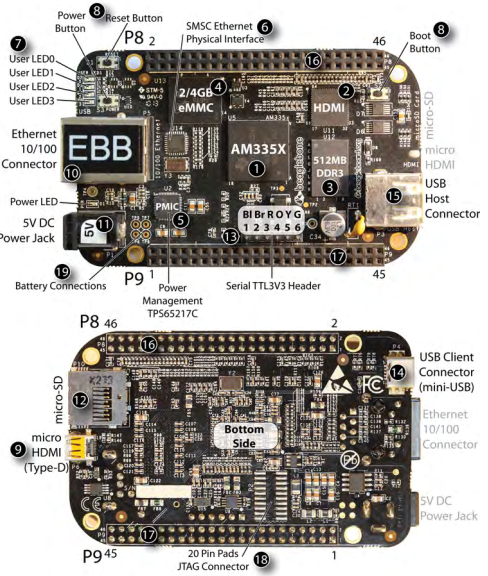
\includegraphics[width=0.6\textwidth]{figuras/bbb_componentes.png}
	\caption{O Beaglebone Black e seus componentes.\cite{derekbbb}}
	\label{figura:bbb_components}
\end{figure}

\begin{figure}
	\centering
	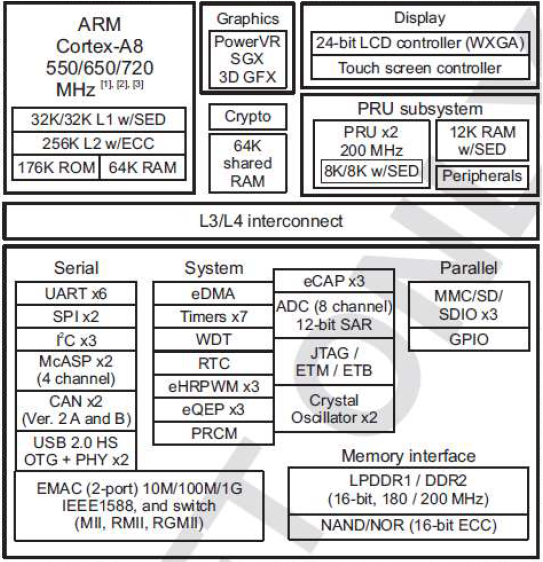
\includegraphics[width=0.6\textwidth]{figuras/bbb_soc.png}
	\caption{Diagrama do Satira AM3358A.\cite{bbbdatasheet}}
	\label{figura:bbb_soc}
\end{figure}

\section{Beaglebone Black e o Linux Embarcado}
\label{ch:bbb_elinux}

Como foi dito nos capítulos anteriores, o Beaglebone Black é um minicomputador completo que é capaz de rodar diversas distribuições de \emph{E-Linux}, Android e outros sistemas operacionais portados para arquitetura ARM. Atualmente a comunidade do Beaglebone portou apenas Android e algumas distribuições Linux, como Debian, Ubuntu, Ångström e Arch Linux. As primeiras versões do Beaglebone Black, mais especificamente as revisões 1 e 2, vinham com Ångström instalado por padrão, uma distribuição linux criada exclusivamente para sistemas embarcados, \emph{tablets}, PDAs, \emph{set top boxes}, roteadores e outros dispositivos baseados na arquitetura ARM \cite{sitebbbang}.

Entretanto, uma parte dos usuários preferiam instalar outra distribuição, como o Ubuntu, pois esta parcela de usuários na maioria das vezes não tinha muita convivência com o Linux e o fato de trabalhar numa distribuição que não tem suas raízes comuns as distrbuições populares para \emph{desktop} tornava o sistema menos amigável. Percebendo a popularidade de tutoriais ensinando como trocar de distribuição, a Texas passou a incluir a distribuição Debian a partir da revisão 3 do Beaglebone Black, lançada em 2014, e revisão mais recente desta placa, além disso, na revisão 3 houve um aumento na memória interna de 2GB para 4GB. Essas adições tornaram o BBB mais atraente para ser usado como computador, pois o espaço extra permitia a instalação de aplicativos para Linux como o \emph{Open Office}, reprodutores de video e editores de imagens.

A nova distribuição facilitou, também, na execução de aplicativos com interface gráfica (GUI) baseados nas \emph{frameworks} GTK+ e Qt, que são bastante populares no Linux \emph{desktop} baseados no Debian e seus derivados, como Ubuntu e Linux Mint. O uso de aplicativos gráficos é bastante comum nas \emph{E-Linux Board} para servir como interface entre o usuário e a máquina. Na figura \ref{figura:bbb_cnc} mostra o exemplo de uma máquina CNC controlada por um Beaglebone e a \emph{cape} K9 CNC I/O. Para controlar a CNC a fabricante da \emph{cape} criou um aplicativo com interface gráfica para Linux onde o usuário é capaz de visualizar o processo e interagir com a CNC.

\begin{figure}[h]
	\centering
	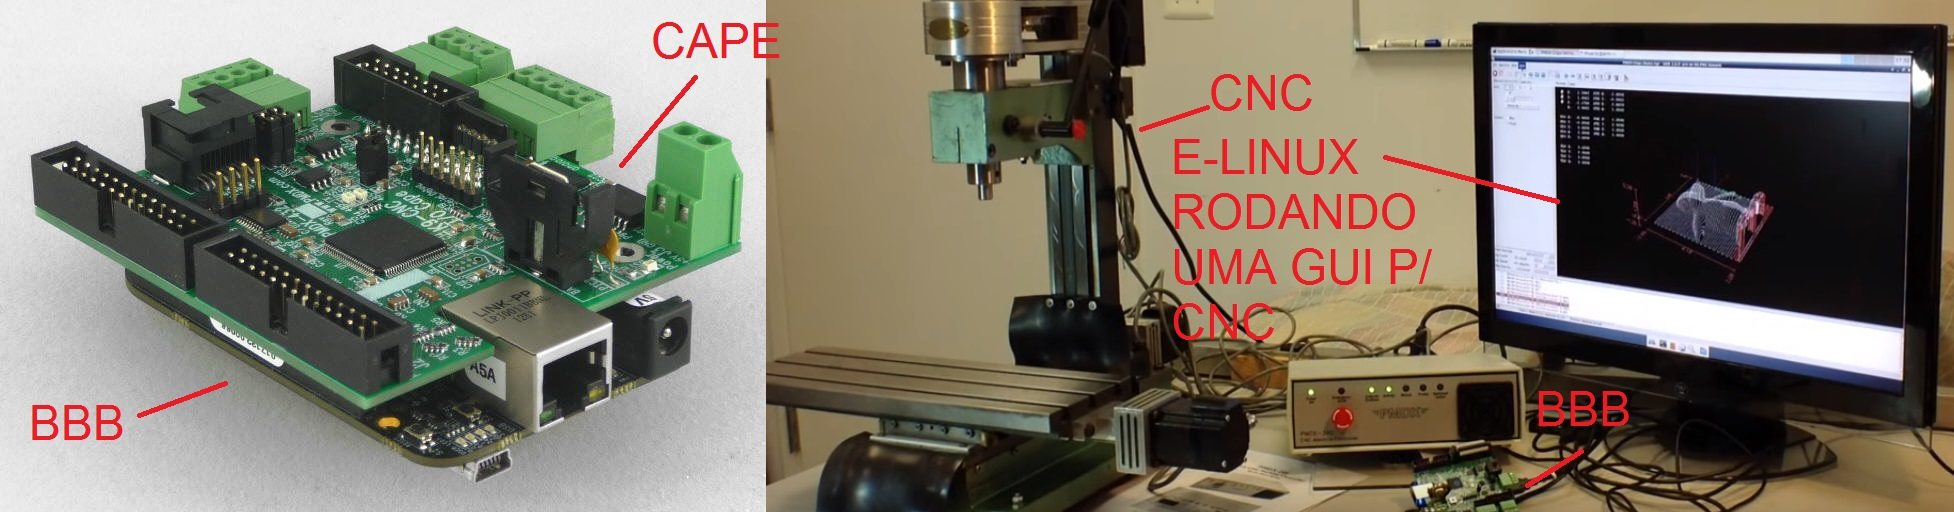
\includegraphics[width=\textwidth]{figuras/cnc_cape.JPG}
	\caption{Beaglebone controlando uma CNC e rodando uma aplicação para CNC simultaneamente.\cite{guicncbbb}}
	\label{figura:bbb_cnc}
\end{figure}

As distribuições baseadas no Debian já vem com as interfaces gráficas e pacotes relacionados instalados por padrão, incluindo aqueles necessários para executar aplicativos criados em Qt ou GTK+. Além disso, essas distribuições vem com diversos outros pacotes que são padrão para a maioria dos usuários Linux, um grande exemplo é o gerenciador de pacotes \emph{apt} que está disponível no Debian, mas não no Ångström.

\subsection{Instalando uma nova distribuição no BBB}

Na seção \ref{ch:bbb_elinux} falo-se da importância de utilizar a distribuição Debian, portanto, se o Beaglebone Black adquirido for anterior a rev.3 deve-se instalar o Debian 7.5 Wheezy, versão de 14/05/2014. Caso o Beaglebone venha uma versão do Debian superior a esta é recomendado fazer o \emph{downgrade} para a versão 7.5, principalmente, se for a versão 8 Jessie ou superior. A versão 7.5 foi projetada pensando, também, nas revisões anteriores a rev. 3, por isso ocupa um pouco menos de 2 Gb, sobrando aproximadamente 2 Gb dos 4Gb da eMMC do BBB, caso este tenha sido adquirido depois de 2014. Esse espaço extra será o suficiente para instalar novos programa, módulos e gerar grandes arquivos de dados. Uma outro motivo fazer o \emph{downgrade} é que neste trabalho e na maioria das bibliografias encontrada na literatura atualmente faz o uso desta versão do Debian, portanto pode haver procedimentos que não sejam os mesmos em versões diferentes, dificultando a reprodução dos experimentos feitos nesta monografia. 

A primeira coisa que deve ser feita para instalar uma nova distribuição é fazer o \emph{download} do sistema operacional, que pode ser baixado na página que contém as  últimas imagens pra Beaglebone Black (\emph{https://beagleboard.org/latest-images}). Caso o leitor desta monografia esteja lendo-a muito tempo depois da sua publicação existe uma alternativa no domínio oficial do Debian (\emph{https://debian.beagleboard.org/images/}), ou ainda, no site do E-Linux (\emph{http://elinux.org/Beagleboard:BeagleBoneBlack\_Debian}). No site das últimas imagens para BBB existem duas versões do Debian 7.5 de 14/05/2014. Uma delas é para utilizar o sistema operacional pelo cartão SD (\emph{without flashing the eMMC}), enquanto a outra grava o sistema operacional na eMMC (\emph{eMMC flasher}). É preferível que o sistema operacional seja instalado na memoria interna do Beaglebone, pois, além desta ter uma taxa de leitura e escrita maior que o cartão SD, ficamos com o \emph{slot} SD livre para ser utilizado em outras ocasiões.

O formato do arquivo baixado é \emph{.img.xz} que é um formato de compactação bastante comum no Linux. Caso o usuário esteja usando o Windows talvez seja necessário fazer o \emph{download} de alguma ferramenta capaz de descompactar este formato de arquivo, visto que alguns aplicativos de descompactação, como WinRar, não trabalham com este tipo de arquivo. Uma sugestão de descompactador capaz de trabalhar com este formato de compactação é o 7-Zip (Disponível em: \emph{http://www.7-zip.org/}), gratuito, \emph{open source} e sem propagandas.

Enquanto a imagem do sistema operacional está sendo baixada, deve-se fazer o \emph{download} de outro programa para gravar a imagem no cartão de memória. Uma sugestão dada pela Wiki do E-Linux é o Win32 Disk Imager (https://sourceforge.net/projects/win32diskimager/) \cite{elinuxupdatebbb}. Quando ambos os arquivos estiverem baixados, descompacte a imagem do Debian que está no formato \emph{.img.xz} e irá obter um arquivo \emph{.img}. Insira o cartão SD no leitor de cartão do seu computador. Abra o Disk Imager selecione a letra correspondente a partição do cartão de memória, selecione a imagem do Debian e clique em gravar como mostra na figura \ref{figura:update_bbb}. Irá aparecer uma caixa de mensagem explicando que esta operação pode danificar os dados no cartão, clique em \emph{yes} espere o processo ser finalizado.

\begin{figure}[h]
	\centering
	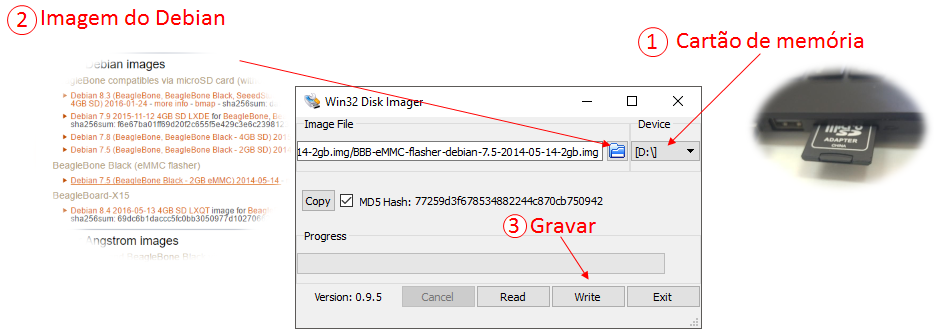
\includegraphics[width=\textwidth]{figuras/update_bbb.png}
	\caption{Gravando a imagem do Debian 7.5 de 14/05/2014 no cartão SD (Próprio Autor)}
	\label{figura:update_bbb}
\end{figure}

Depois do processo de gravação finalizar com sucesso retire o cartão SD do cartão e com o BBB ainda desligado, insira o microSD no \emph{slot} apropriado (Item 12 na figura \ref{figura:bbb_components}). Antes de ligar a placa, mantenha pressionado o \emph{Boot Switch} (Item 8 na figura \ref{figura:bbb_components}), e ainda com o botão pressionado, conecte a porta USB \emph{Client} do Beaglebone (Item 14 na figura \ref{figura:bbb_components}) e ao computador ou alguma fonte de alimentação. Depois dos \emph{User LEDs} (Item 7 na figura \ref{figura:bbb_components}) começarem a piscar solte o \emph{Boot Switch}. A partir daí, o sistema operacional será instalado na eMMC o processo dura cerca de 30 a 40 minutos, durante este tempo não desligue o Beaglebone. Quando a instalação estiver concluída os 4 \emph{User LEDs} irão parar de piscar e ficarão acesos. Neste momento desconecte oo cabo USB da fonte de alimentação retire o cartão SD e conecte novamente o BBB ao computador. Será montada uma partição FAT com o nome \emph{BeagleBone Getting Started} clique nela e abra o arquivo \emph{ID.txt} com o bloco de notas. Se aparecer \emph{BeagleBoard.org BeagleBone Debian Image 2014-04-23
} a atualização da Distro foi realizada com sucesso (Figura \ref{figura:check_bbb_version}).

\begin{figure}[h]
	\centering
	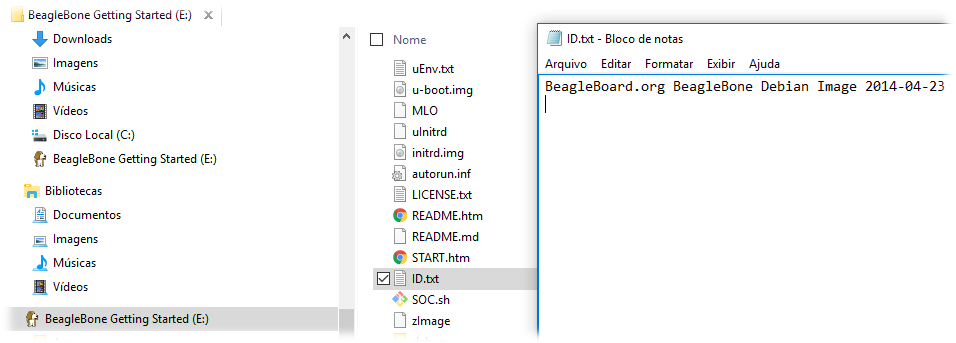
\includegraphics[width=\textwidth]{figuras/check_bbb_version.png}
	\caption{Verificando a atualização do Debian 7.5 foi instalada com sucesso. (Próprio Autor)}
	\label{figura:check_bbb_version}
\end{figure}

\subsection{Comunicando com o BeagleBone Black}

O Beaglebone Black \emph{vanilla}, ou seja, da forma como veio de fábrica, não tem nenhuma interface de interação com o usuário além de alguns \emph{push-bottons} e LEDs indicadores (Itens 7 e 8 da figura \ref{figura:bbb_components}). E isso não é o suficiente para programar ou adicionar alguma nova função a placa de desenvolvimento, a menos que o usuário use o BeagleBone ligado a um monitor, mouse e teclado. Para interagir com o \emph{board computer} sem a necessidade desses aparelhos é necessário se comunicar com o BBB através de um computador hospedeiro. Existem diversas formas de fazer esta comunicação, mas esta seção irá focar na protocolo SSH e no \emph{serial debug}.

$$Vem uma figura aqui$$

O Linux, Mac e sistemas operacionais baseados no Unix, já vem com suporte nativo a SSH através do terminal. Usuários do Windows podem experimentar o \emph{Windows 10 bash shelll}, porém esta solução no momento  , entretanto, usuários do Windows devem baixar um cliente SSH como o PuTTY (Disponível em: \emph{http://www.putty.org/}). Antes de iniciar o processo de comunicação é importante atualizar os \emph{drivers} disponivel em: \emph{http://beagleboard.org/static/beaglebone/latest/README.htm}. Depois da atualização feita e o PuTTY baixado abra este último aplicativo. No campo \emph{Host Name (or IP address)} escreva o IP do BeagleBone que por padrão é $192.168.7.2$. Deixe as outras opções padrões como mostra a figura \ref{}


\subsection{Programando no BeagleBone Black}
\label{ch:bbb_firststeps}

O fato do BeagleBone Black utilizar Linux como sistema operacional o usuário programe em uma infinidade de linguagens de programação, entretanto algumas delas necessitam de passos adicionais. Esta que não vêm instaladas por padrão não serão abordadas nesta seção.

Ao conectar o Beaglebone Black ao computador através da porta USB Client (Item 14 na figura\ref{figura:bbb_components}) será montada a partição FAT \emph{BeagleBone Getting Star


Nas seções anteriores vimos os componentes do BBB e 

Como foi dito na seção \

O fato do BBB já vim com o linux embarcado permite que possa programar em 